%scritto da \PF{}
\subsubsection{UCA 4 - Inserimento modalità di tracciamento}%kite level

\begin{figure}[h]
	\centering	
	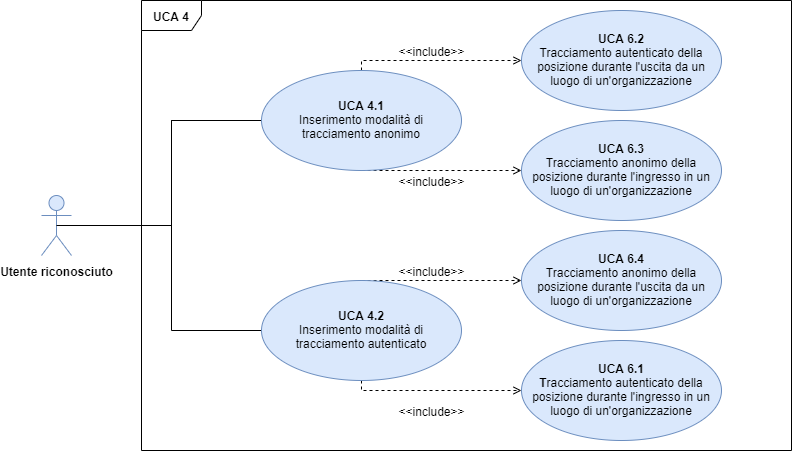
\includegraphics[scale=0.53, center]{Sezioni/UseCase/Immagini/UCA4.png}
	\caption{UCA 4 - Inserimento modalità di tracciamento}
\end{figure}

\begin{itemize}
	\item \textbf{Attori primari:} Utente riconosciuto
	\item \textbf{Precondizione:} L'utente si è autenticato con le credenziali \glo{LDAP} nella \glo{organizzazione} in cui si trova e vuole selezionare la modalità di \glo{tracciamento}.
	\item \textbf{Postcondizione:} L'utente viene tracciato secondo la modalità da lui scelta precedentemente.
	\item \textbf{Scenario principale:} L'utente accede alla funzionalità di selezione della modalità di \glo{tracciamento}.
	\item \textbf{Flusso di eventi:}
	\begin{enumerate}
		\item L'utente accede alla funzione di inserimento modalità di tracciamento;
		\item L'utente può scegliere la modalità di \glo{tracciamento anonimo} [UCA 4.1] oppure la modalità di \glo{tracciamento autenticato} [UCA 4.2].
	\end{enumerate}
\end{itemize}

\subsubsection{UCA 4.1 - Inserimento modalità di tracciamento anonimo}%sea level
\begin{itemize}
	\item \textbf{Attori primari:} Utente riconosciuto
	\item \textbf{Precondizione:} L'utente si è autenticato con le credenziali \glo{LDAP} nella \glo{organizzazione} in cui si trova e vuole selezionare la modalità di tracciamento anonimo].
	\item \textbf{Postcondizione:} L'utente viene tracciato secondo la \glo{modalità di tracciamento anonimo}.
	\item \textbf{Scenario principale:} L'utente accede alla funzionalità inserimento modalità di \glo{tracciamento} e inserisce la \glo{modalità di tracciamento anonimo}.
	\item \textbf{Flusso di eventi:}
	\begin{enumerate}
	\item L'utente accede alla funzione di inserimento \glo{modalità di tracciamento anonimo};
	\item L'utente inserisce la \glo{modalità di tracciamento anonimo};
	\item Viene inviata al sistema l'uscita dell'utente autenticato dall'\glo{organizzazione} [UCA 6.2];
	\item Viene inviato al sistema l'entrata dell'utente anonimo nell'\glo{organizzazione} [UCA 6.3].
	\end{enumerate}
	\item \textbf{Inclusioni:}
	\begin{itemize}
		\item UCA 6.2 - \glo{Tracciamento autenticato} della posizione durante l'uscita da un luogo di un'\glo{organizzazione};
		\item UCA 6.3 - \glo{Tracciamento anonimo} della posizione durante l'ingresso in un luogo di un'\glo{organizzazione}.
	\end{itemize}
\end{itemize}

\subsubsection{UCA 4.2 - Inserimento modalità di \glo{tracciamento autenticato}}%sea level
\begin{itemize}
	\item \textbf{Attori primari:} Utente riconosciuto
	\item \textbf{Precondizione:} L'utente si è autenticato con le credenziali \glo{LDAP} nella \glo{organizzazione} in cui si trova e vuole selezionare la modalità di \glo{tracciamento autenticato}.
	\item \textbf{Postcondizione:} L'utente viene tracciato secondo la \glo{modalità di tracciamento anonimo}.
	\item \textbf{Scenario principale:} L'utente accede alla funzionalità inserimento modalità di \glo{tracciamento} e inserisce la \glo{modalità di tracciamento autenticato}.
	\begin{enumerate}
		\item L'utente accede alla funzione di inserimento modalità di \glo{tracciamento autenticato};
		\item L'utente inserisce la modalità di \glo{tracciamento autenticato};
		\item Viene inviata al sistema l'uscita dell'utente anonimo dall'\glo{organizzazione} [UCA 6.4];
		\item Viene inviato al sistema l'entrata dell'utente autenticato nell'\glo{organizzazione} [UCA 6.1].
	\end{enumerate}
	\begin{itemize}
		\item UCA 6.4 - Tracciamento anonimo della posizione durante l'uscita da un luogo di un'organizzazione;
		\item UCA 6.1 - Tracciamento autenticato della posizione durante l'ingresso in un luogo di un'organizzazione.
	\end{itemize}
\end{itemize}
